\begin{frame}
	\frametitle{Accounting for Neighbouring Structures}
	
	By construction, the identified subhalos are not isolated. 
	This fact changes the situation significantly for the interpretation of what particles should be considered bound.
	
	Consider first a particle $\alpha$ in the potential of an isolated clump:
	
	
	\begin{figure}
		\centering
		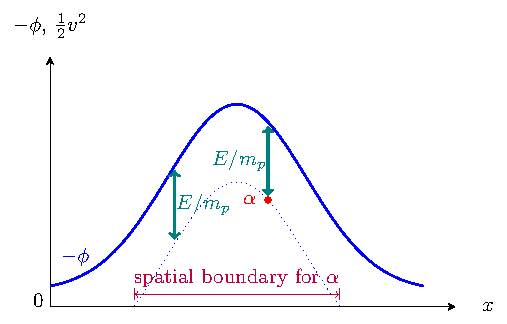
\includegraphics[width=.7\textwidth]{../report/images/tikz/boundaries.pdf}
	\end{figure}
	
	
	The spatial boundaries of its trajectory can be found by demanding energy conservation
	$	E/m_p = \frac{1}{2} v^2 + \phi = const.	$
	by following the curve of constant total energy to the points where $v^2 =0$. 
\end{frame}








\begin{frame}
	\frametitle{Accounting for Neighbouring Structures}
	
	Now apply the same thoughts to an isolated halo that is made up from two clumps:
	
	
	\begin{figure}
		\centering
		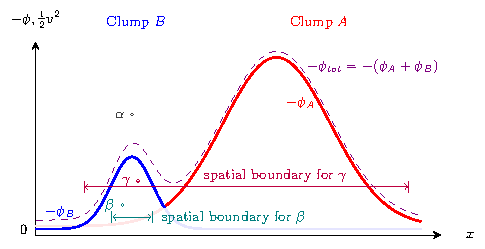
\includegraphics[width=.8\textwidth]{../report/images/tikz/potentials.pdf}
	\end{figure}
	
	\begin{itemize}
		\small
		\item $\alpha$ is clearly not bound to the clump $B$.
		\item $\beta$ will remain bound on an elliptic trajectory around the centre of mass.
		\item $\gamma$ is energetically bound to the clump just like $\beta$, but because of clump $A$'s neighbouring potential, the particle can leave the boundaries of clump $B$ and wander off deep into clump $A$.
	\end{itemize}
	

\end{frame}








\begin{frame}
	\frametitle{Accounting for Neighbouring Structures}
	
	\begin{columns}
		\column{.7\textwidth}
			$\Rightarrow$ Particles like $\gamma$ shouldn't be considered bound.
			
			The reason $\gamma$ can wander off is because its boundary extends past the interface that connects the two clumps
			
			$\Rightarrow$ the condition for a particle to be \emph{exclusively} bound must be that its trajectory must never reach that interface.
				
		\column{.3\textwidth}
			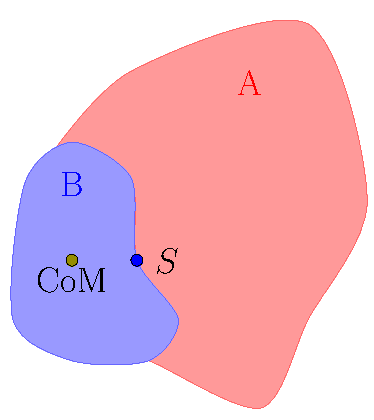
\includegraphics[width=\textwidth]{./images/tikz/saddle.pdf}
			\vspace{1cm}
	\end{columns}

	
	$\Rightarrow$ Define $S$ to be the point on the interface to the neighbouring structure(s) that is closest to B’s centre of mass and $\phi_S$ to be the potential of clump $B$ at that point. Using the same argumentation as before, a particle can't reach $S$ if 
	\begin{align*}
	v < \sqrt{ - 2(\phi - \phi_S) } 
	\end{align*}
	
\end{frame}







\begin{frame}
	\frametitle{Results: \dt-dataset}
	
	\begin{tabular}{c c}
		\simple\ 	& \neigh \\[1.5em]
		%
		%	 
		{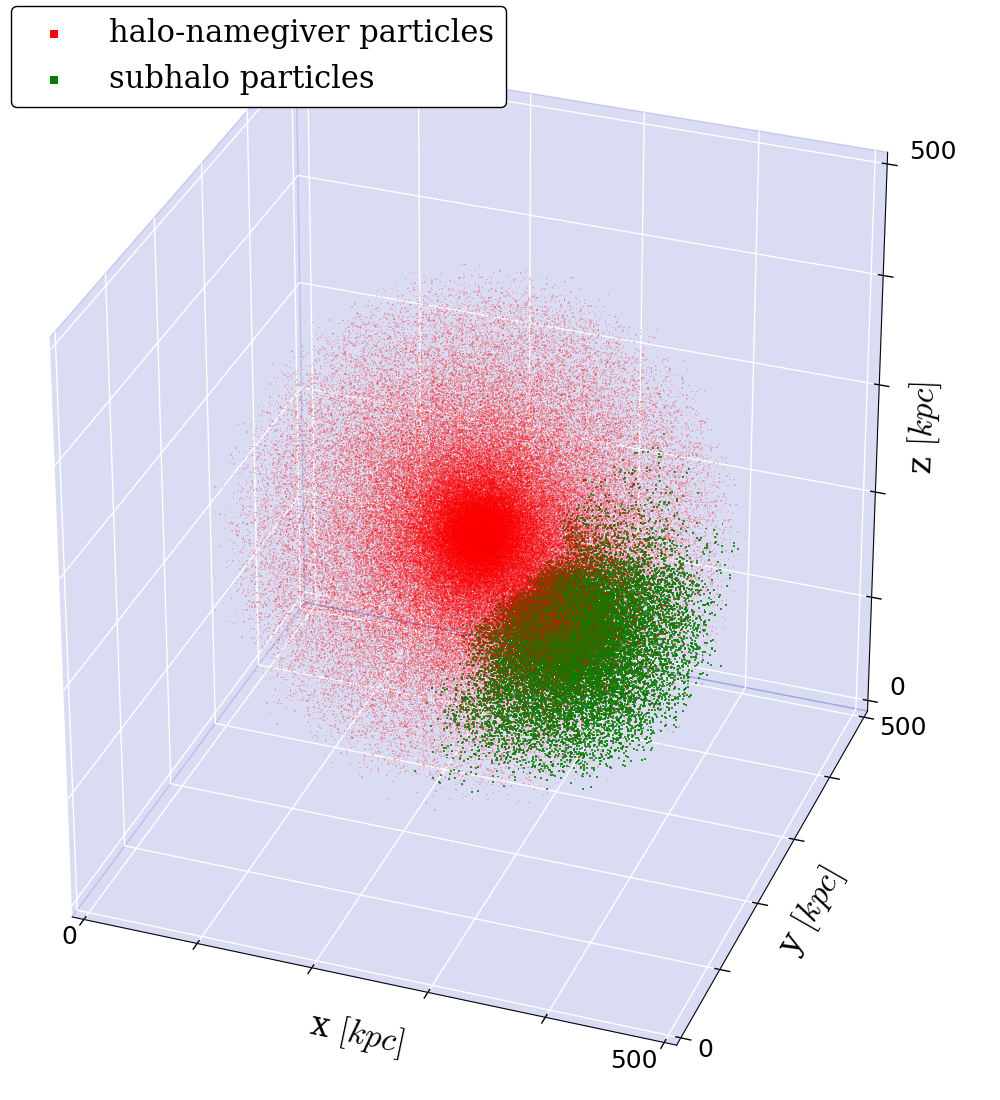
\includegraphics[width = .49\textwidth]{../report/images/dice-two/dice-two-plot-halo1451-nosaddle.png}} &
		{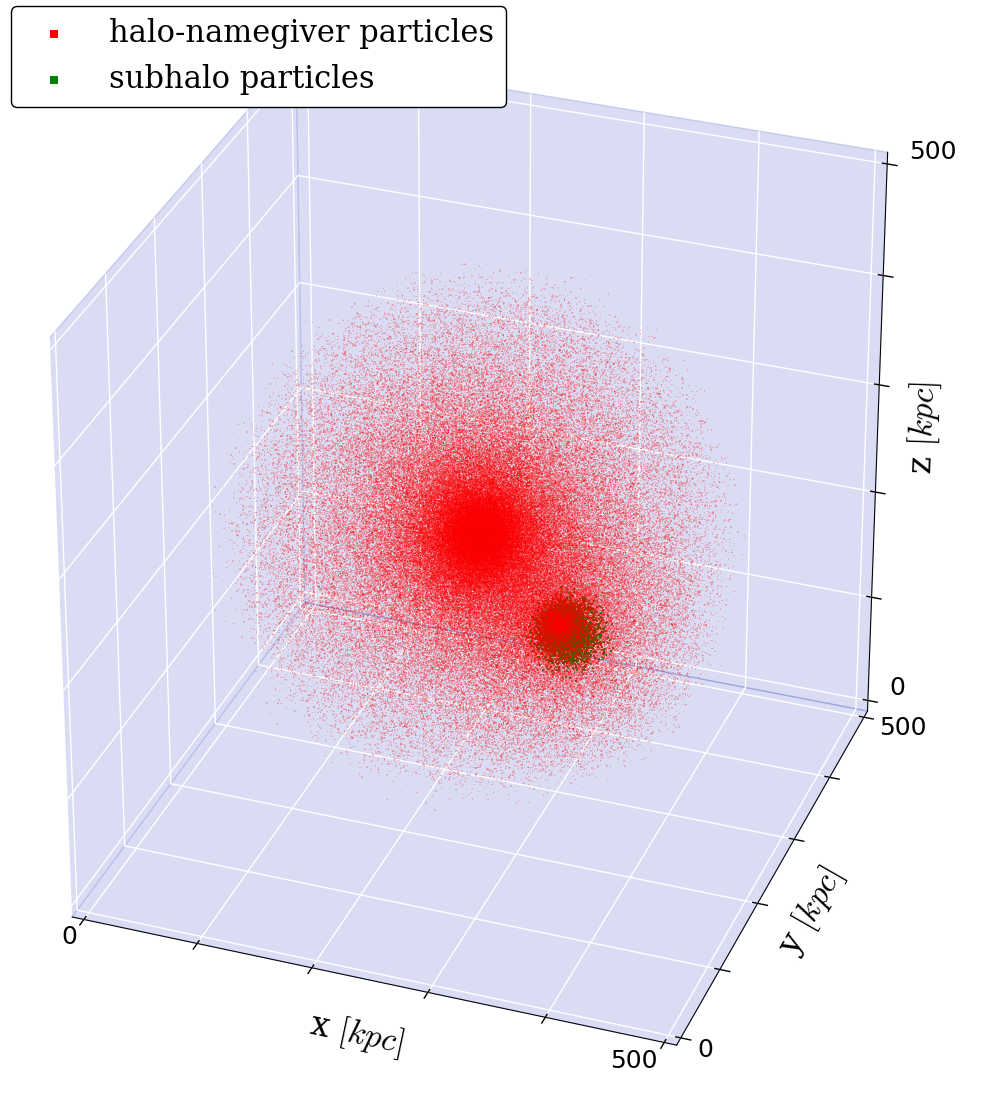
\includegraphics[width = .49\textwidth]{../report/images/dice-two/dice-two-plot-halo1451-saddle.png}} \hspace*{-1em} 
	\end{tabular}
\end{frame}





\begin{frame}
	\frametitle{Results: \dt-dataset: subhalo particles only}
	
	\begin{tabular}{c c}
		\simple\ 	& \neigh \\[1.5em]
		%
		%	 
		{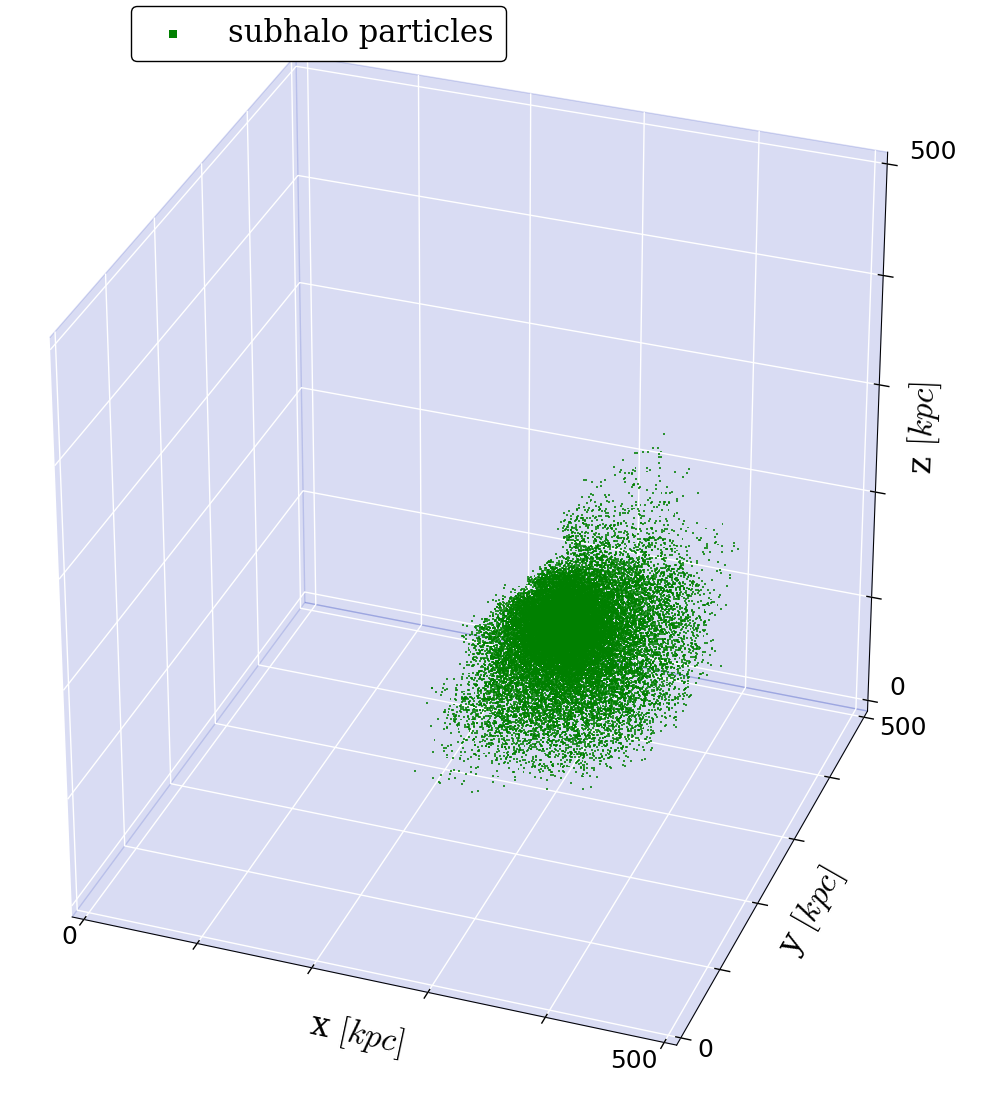
\includegraphics[width = .49\textwidth]{../report/images/dice-two/dice-two-plot-subhalo-nosaddle.png}}	&
		{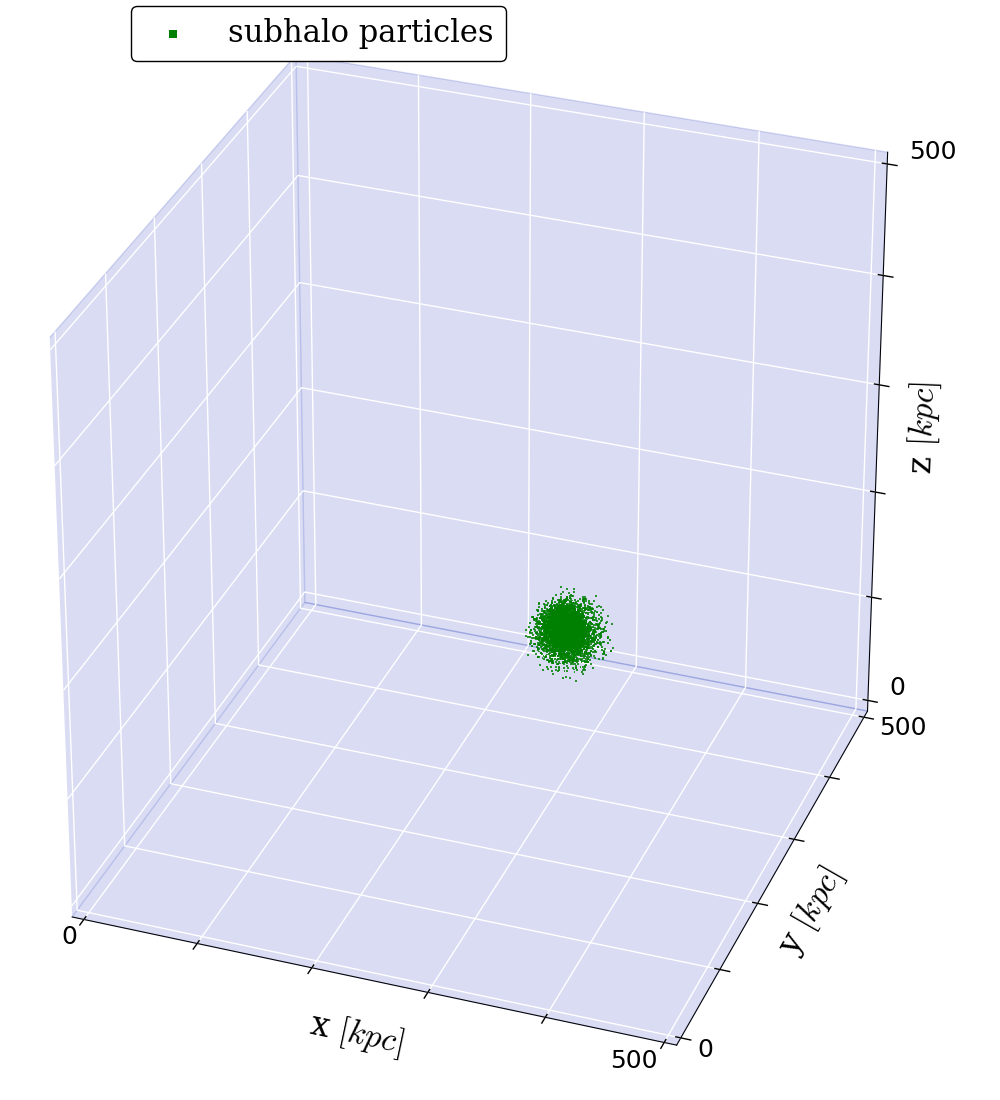
\includegraphics[width = .49\textwidth]{../report/images/dice-two/dice-two-plot-subhalo-saddle.png}}  
	\end{tabular}
\end{frame}




%\begin{frame}
%	\frametitle{Results: \ds-dataset}
%	
%	\begin{tabular}{c c}
%		\simple\ 	& \neigh \\[1.5em]
%		%
%		%
%		 
%		{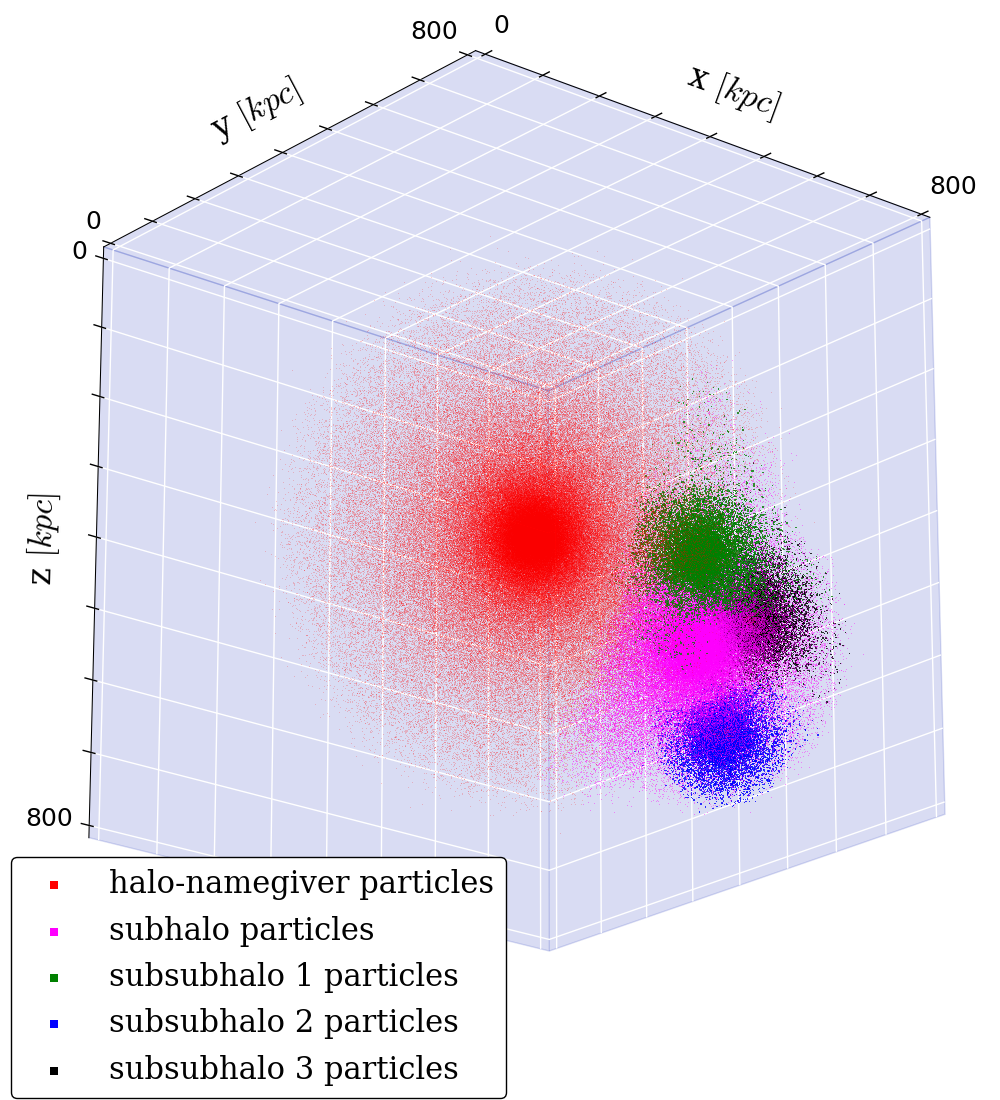
\includegraphics[width = .49\textwidth]{../report/images/dice-sub/dice-sub-plot-halo1-nosaddle.png}}	&		 
%		{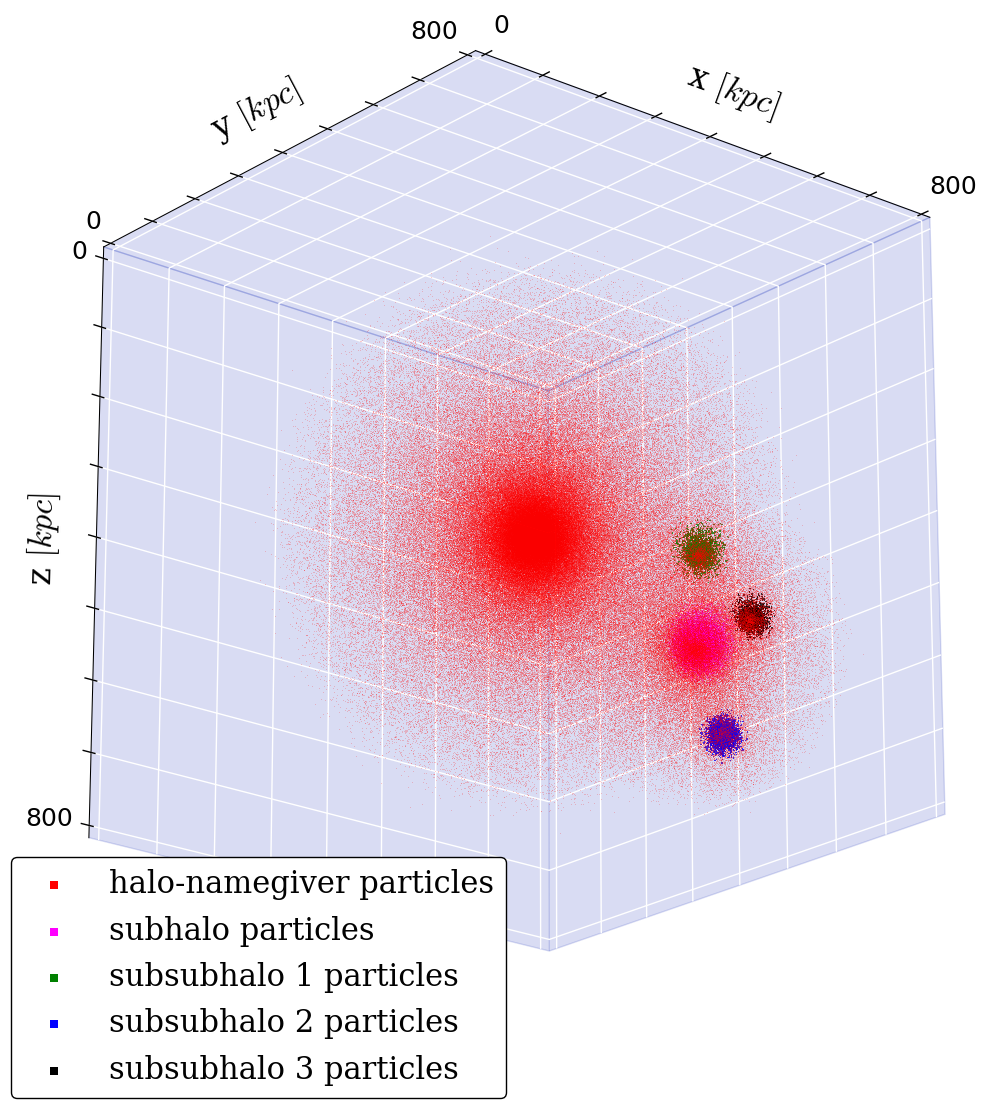
\includegraphics[width = .49\textwidth]{../report/images/dice-sub/dice-sub-plot-halo1-saddle.png}} 	
%	\end{tabular}
%\end{frame}
%
%
%
%\begin{frame}
%	\frametitle{Results: \ds-dataset: halo-namegiver particles only}
%	
%	\begin{tabular}{c c}
%		\simple\ 	& \neigh \\[1.5em]
%		%
%		%	 
%		{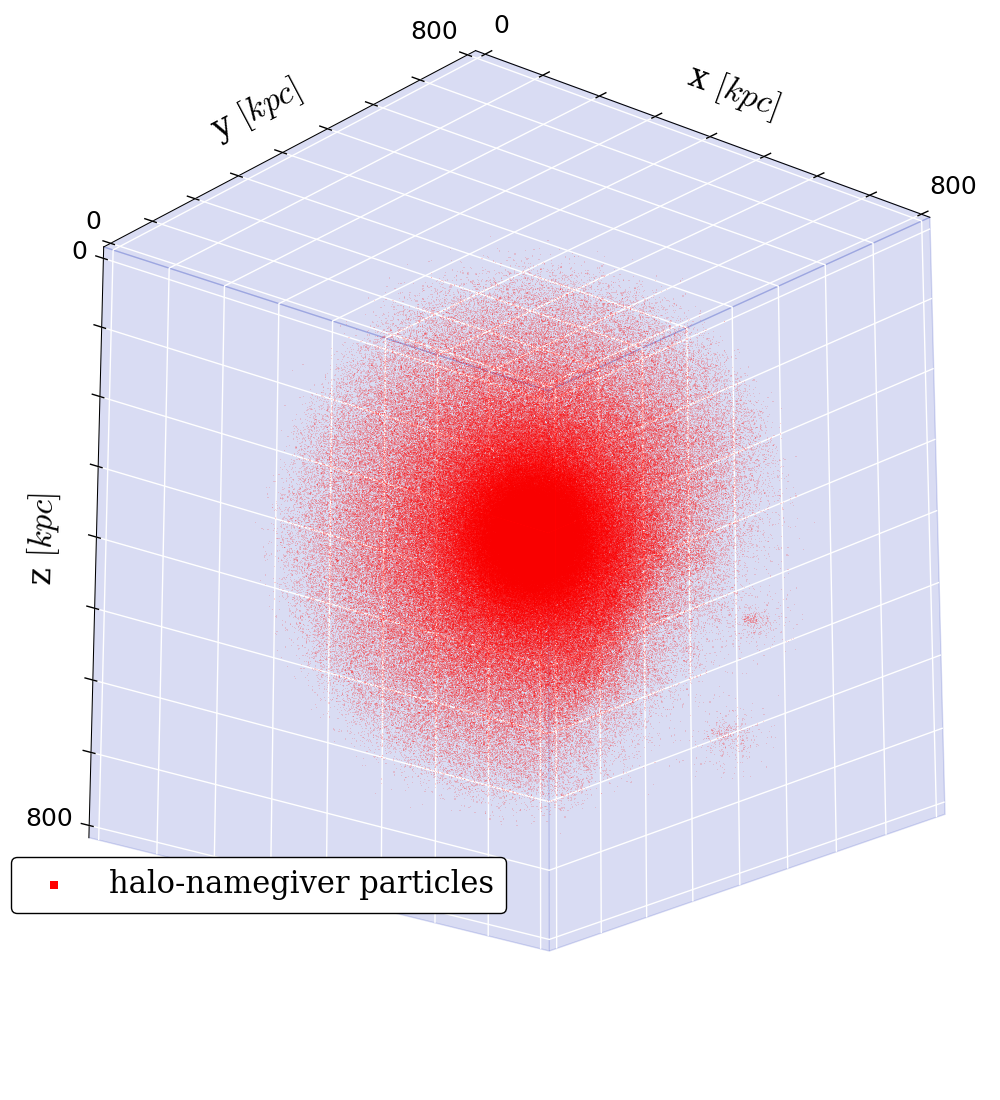
\includegraphics[width = .49\textwidth]{../report/images/dice-sub/dice-sub-halo-only-nosaddle.png}} \hspace*{-1em} 	& 
%		{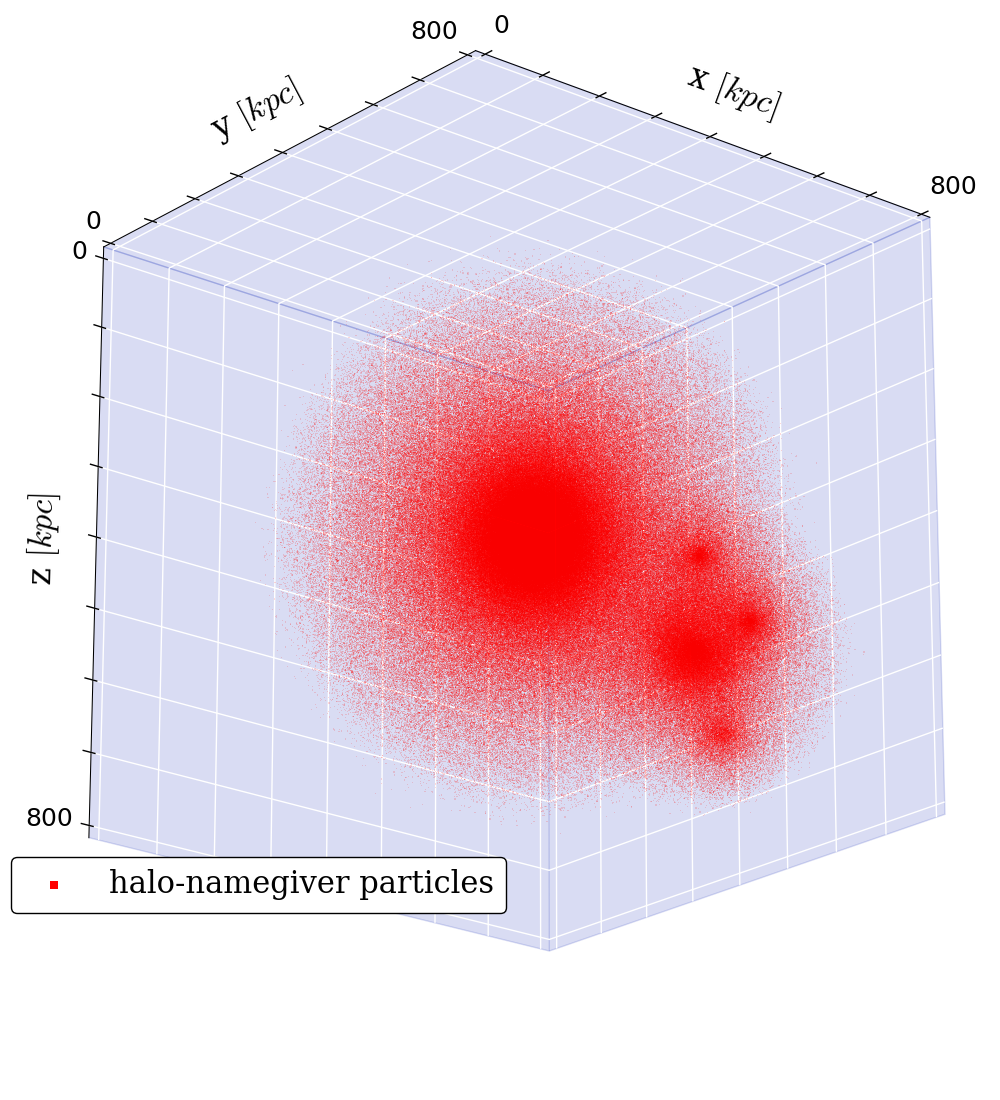
\includegraphics[width = .49\textwidth]{../report/images/dice-sub/dice-sub-halo-only-saddle.png}}
%	\end{tabular}
%\end{frame}



\begin{frame}
	\frametitle{Results: \cosmo-dataset}
	
	\begin{tabular}{c c}
		\simple\ 	& \neigh \\[1.5em]
		%
		%	 
		{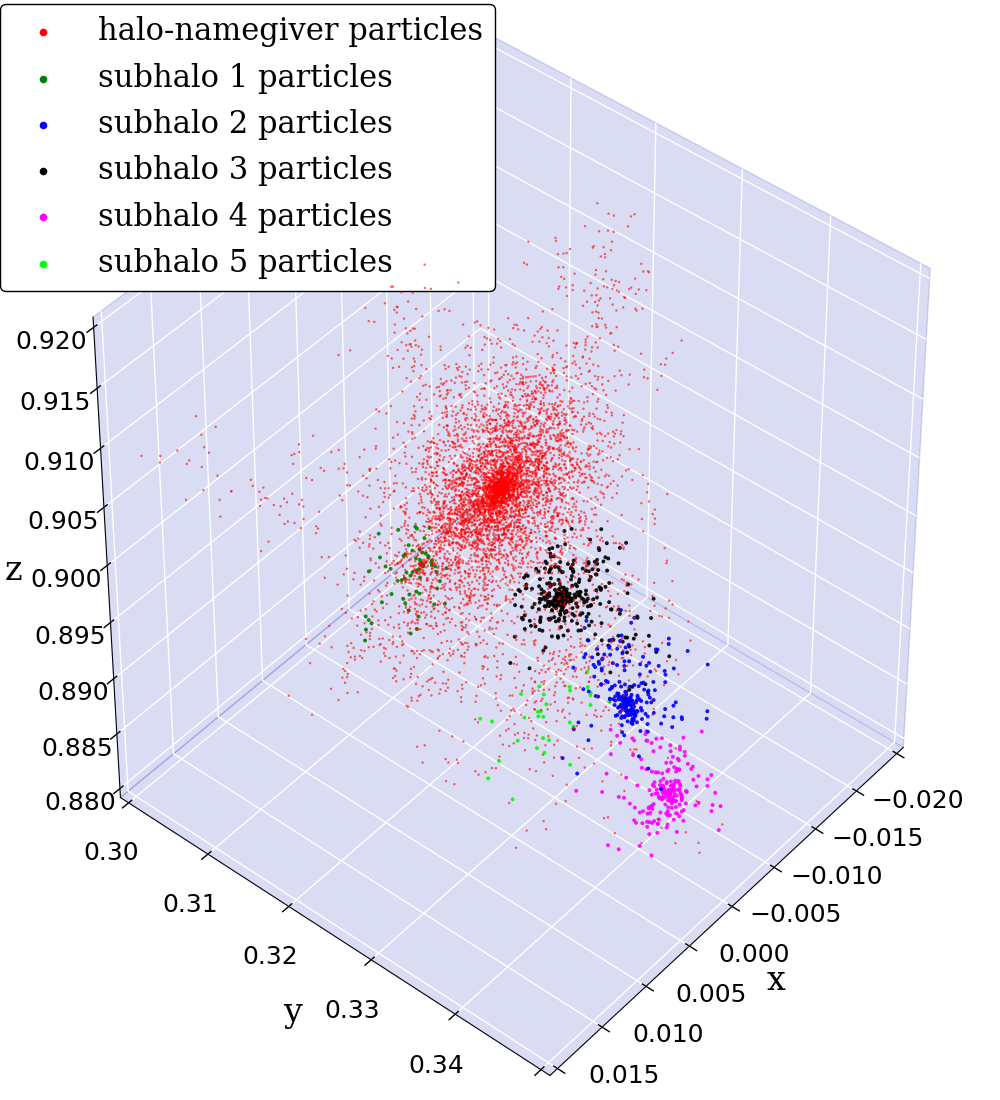
\includegraphics[width = .49\textwidth]{../report/images/cosmo/cos-halo-66858-nosaddle.png}}	& 
		{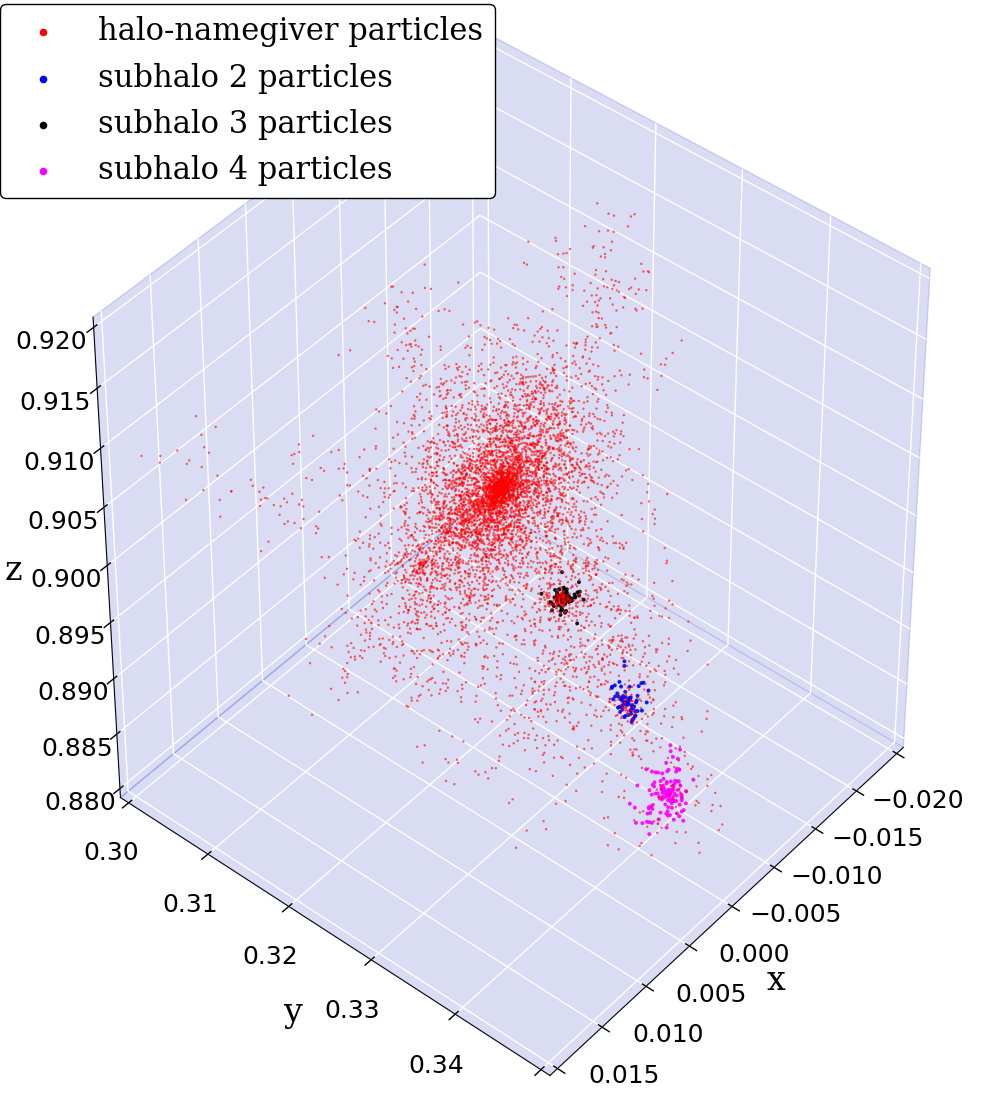
\includegraphics[width = .49\textwidth]{../report/images/cosmo/cos-halo-66858-saddle.png}}
	\end{tabular}
\end{frame}



\begin{frame}
	\frametitle{Results: \cosmo-dataset: subhalo particles only}
	
	\begin{tabular}{c c}
		\simple\ 	& \neigh \\[1.5em]
		%
		%	 
		{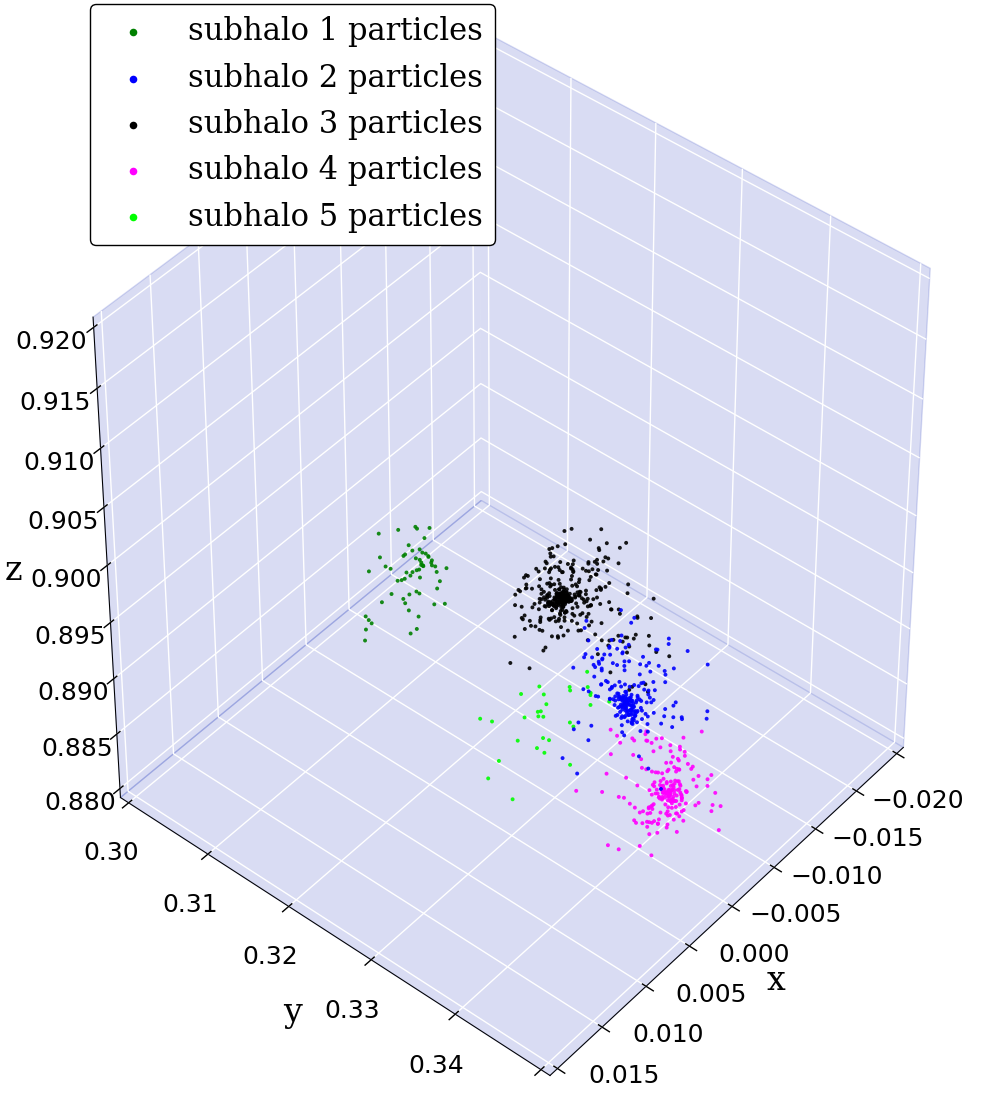
\includegraphics[width = .49\textwidth]{../report/images/cosmo/cos-halo-66858-subhalo-only-nosaddle.png}} \hspace*{-1em} 	& 
		{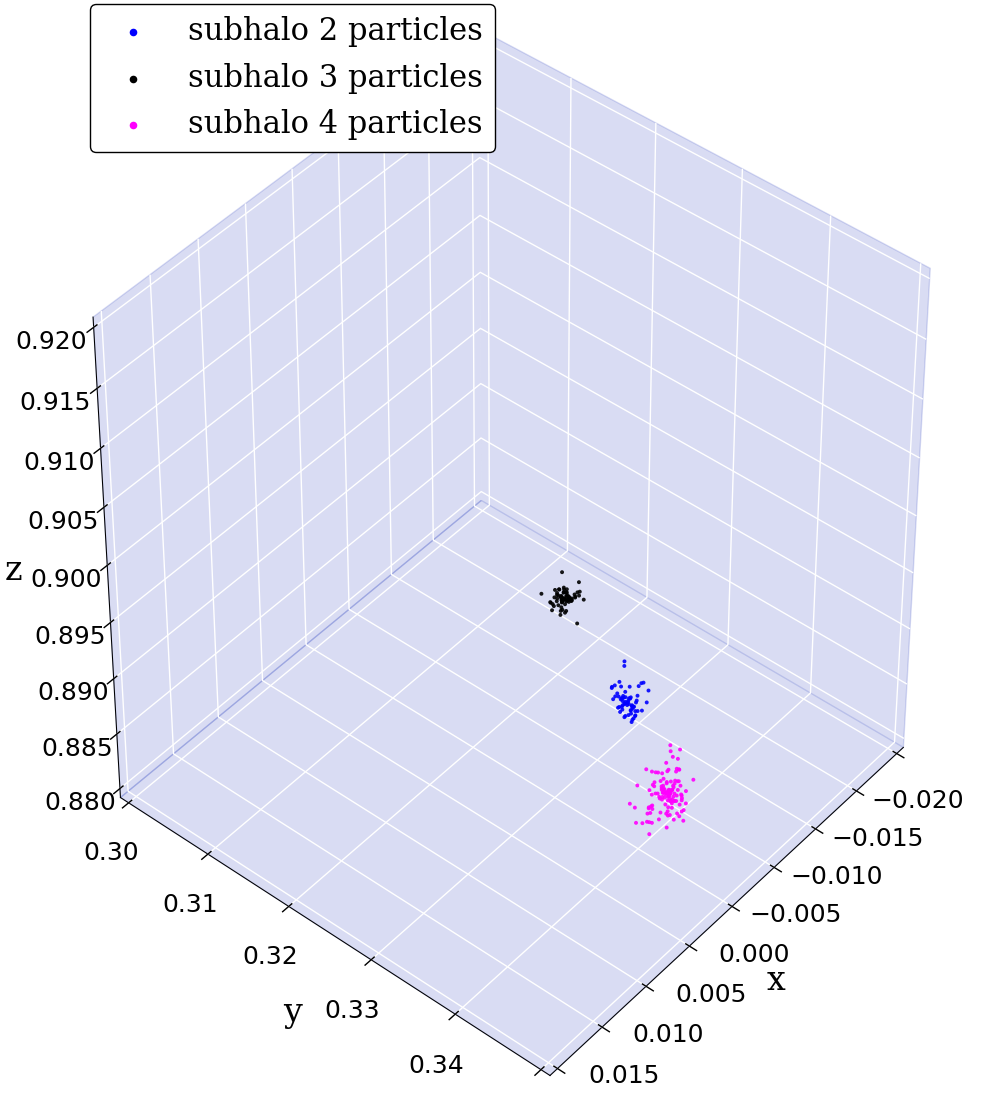
\includegraphics[width = .49\textwidth]{../report/images/cosmo/cos-halo-66858-subhalo-only-saddle.png}}
	\end{tabular}
\end{frame}